\documentclass[twoside, a4paper, twocolumn, reqno]{article}
\usepackage[english]{babel}
\usepackage{a4wide}

\usepackage{ics}

% Fonts
\usepackage[sc]{mathpazo}
\usepackage[T1]{fontenc}
\linespread{1.05}
\usepackage{lmodern}
\usepackage{microtype}
\usepackage{lettrine}

% Document layout
% \usepackage[hmarginratio=1:1,top=32mm,columnsep=20pt]{geometry}
\usepackage{paralist}

% Floats
\usepackage{float}

%Plaatjes
\usepackage{tikz}
\usepackage{graphicx}
\usepackage[small, labelfont=bf, up, textfont=sl, up, justification=raggedright]{caption}
\usepackage{subcaption}
\DeclareCaptionLabelFormat{opening}{(#2)}
\captionsetup{subrefformat=opening}

% Tables
\usepackage{booktabs}

% Custom section headers
\usepackage{titlesec}
\titleformat{\section}[block]{\large\scshape}{\thesection.}{1em}{}
\titleformat{\subsection}[block]{\large\scshape}{\thesubsection.}{1em}{}
\titleformat{\subsubsection}[block]{\scshape}{\thesubsubsection.}{1em}{}

%Wiskunde
\usepackage[scientific-notation=true, round-mode=figures, round-precision=3, exponent-base=e, exponent-product={}]{siunitx}
\usepackage{mathtools}
\usepackage{amsmath}
\usepackage{amsfonts}
\usepackage{amssymb}

% References
\usepackage{varioref}
\usepackage{hyperref}
\usepackage[noabbrev, capitalize]{cleveref}

% References
\usepackage[backend=bibtex]{biblatex}
\usepackage{csquotes}
\bibliography{biblio}

% Pseudo code
\usepackage[algoruled,vlined, shortend]{algorithm2e}
\usepackage[export]{adjustbox}
\usepackage{setspace}

\crefname{algocf}{algorithm}{algorithms}
\Crefname{algocf}{Algorithm}{Algorithms}
\crefname{algocfline}{line}{lines}
\Crefname{algocfline}{Line}{Lines}

% Temp
\usepackage[obeyFinal]{todonotes}
% \usepackage{showlabels}
\newcommand{\laura}[1]{\todo[inline, color=red]{\textbf{Laura:} #1}}
\newcommand{\rick}[1]{\todo[inline, color=green]{\textbf{Rick:} #1}}
\newcommand{\future}[1]{\todo[inline, color=yellow]{\textbf{Possibly eventually:} #1}}
\newcommand{\plaatje}[1]{\todo[inline, color=blue!20]{\textbf{Plaatje:} #1}}
\newcommand{\ooit}[1]{\todo[inline, color=green!20]{\textbf{(n)ooit:} #1}}

% Math commands
\newcommand{\normal}[2]{\ensuremath{\mathcal{N}\left(#1,\, #2\right)}}
% \renewcommand{\vec}[1]{\ensuremath{\mathbf{#1}}}
\usepackage{mathtools}

\DeclarePairedDelimiter\abs{\lvert}{\rvert}%
\DeclarePairedDelimiter\norm{\lVert}{\rVert}%

% Swap the definition of \abs* and \norm*, so that \abs
% and \norm resizes the size of the brackets, and the 
% starred version does not.
\makeatletter
\let\oldabs\abs
\def\abs{\@ifstar{\oldabs}{\oldabs*}}
%
\let\oldnorm\norm
\def\norm{\@ifstar{\oldnorm}{\oldnorm*}}
\makeatother
% Lists
\usepackage{paralist}

% Other commands
\renewcommand{\t}[1]{\texttt{#1}}

\title{A Spring Simulation of Crack Dynamics}
\author{%
	Rick van Veen (s1883933)%
	\thanks{These authors contributed equally to this work.}% 
	\and% 
	Laura Baakman (s1869140)%
	\footnotemark[1]%
}

\begin{document}

\maketitle

\section{Introduction}
\label{s:introduction}
%!TEX root = report.tex
One of the major difficulties in modeling the transport of solutes as well as the flow of water, is the dynamics of the formation of cracks in clay soils. These networks of macro pores are governed by the dessication process. Modern simulations of the flow of water and the transport of dissolved matter are capable of modeling the flow of water within these pores \cite{vogel2005studies2}.

In general models of the dynamics of soil, cracks focus on properties of the network of cracks in general, e.g., the volume as a function of water content and soil depth \cite{chertkov2000using}. However as these models completely disregard the geometry of the network of cracks they are not suitable for use in state-of-the-art models the flow of water and solutes. Other models, such as the one introduced by \textcite{horgan2000empirical}, take the geometry of the network into account but do not model the process of crack formation realistically. 

\textcite{kitsunezaki1999fracture} models the formation of cracks in one dimension as a chain of particles, connected to their two neighbors by horizontal springs and grounded by vertical springs. By decreasing the natural length of the springs they simulate the shrinking of the material. Springs break if their energy exceeds some critical value. \citeauthor{kitsunezaki1999fracture} determines the horizontal displacements of particles by minimizing some energy function. 

A model with some of the same ideas has been introduced by \textcite{vogel2005studies2}. Contrary to \citeauthor{kitsunezaki1999fracture}, \citeauthor{vogel2005studies2} use a two-dimensional lattice with ungrounded Hookean springs whose natural length decreases, i.e., there are no vertical springs connecting the lattice to some basis.  The condition under which springs break is similar to the one used by \citeauthor{kitsunezaki1999fracture}. The change resulting from a broken spring is propagated radially throughout the lattice until a maximum number of steps has been taken, or the system has stabilized completely. The resulting model realistically represents the process of crack formation. Furthermore the model's properties can be directly linked to the physical properties and boundary conditions of the material.

We propose a simplified model based on that introduced by \citeauthor{vogel2005studies2}, that although not as representative of prominent features physical can be solved faster and should give a reasonable indication of crack dynamics. Our model represents the particles and the springs between them as a linear model. This allows us to use a linear solver to determine the new positions of the particles after springs have been broken. In this newly stabilized system we once again break springs. The steps of stabilizing the network and breaking springs are repeated until no more springs can be broken, be it because there are no more springs left, or because there are no more springs that satisfy the requirement for being broken. The repeated stabilization and breaking of springs models the dessication of the material.

\Cref{s:method} presents the theory of our method. The implementation the simulation based on the discussed method is introduced in \cref{s:implementation}. \Cref{s:ExperimentsDiscussion} presents the experiments we performed with our implementation and presents and reviews the gathered results. Finally, \cref{s:conclusion} discusses our conclusion.

\section{Method}
\label{s:method}
%!TEX root = report.tex

\todo[inline]{Intro plus what one can find in this section... }
When simulating the dynamics of cracking material, one needs a model that represents the properties of that materials, mud in our case. In \cref{ss:method:model} we present our model. \Cref{ss:method:vogel} presents the model introduced by \citeauthor{vogel2005studies2} on which ours is loosely based. So that we can contrast the two models in \cref{ss:method:contrast}.

\subsection{The model}\label{ss:method:model}
% \todo[inline]{``Decribe our model:  1. Properties of single particles and connection between two (springs)''}
We use a spring simulation to model the rupture dynamics of mud. In this section we first describe the behavior and properties of one spring connecting two particles. \todo{Wat doen we in de rest van deze sectie}

Since the cracking of mud is a very slow process we can ignore Newton's and Stokes' law, i.e., we do not consider the effect of velocity and frictional forces in our model. Consequently our particles are massless and we only consider their location. This, and some other properties of our model, make it possible to find the new position of particles using a matrix vector equation, which can be solved with a linear solver.

\begin{figure}
	\centering
	  \begin{tikzpicture}
	    \node [free]  (left)  at  (0,0)   {\freeParticle{i}};
	    \node [free]  (right)   at  (4,0) {\freeParticle{j}};
	    \drawSpring{left}{right}{0}

	    \node (leftUpper) at (0,0.5) {};
	    \node (rightUpper) at (4,0.5) {};
	    \draw[dashed, <->] (leftUpper)--(rightUpper) node[foo] {$D_{ij} = \abs{x_i - x_j}$};

	    \node (leftLower) at (1,-0.5) {};
	    \node (rightLower) at (3,-0.5) {};
	    \draw[dashed, <->] (leftLower)--(rightLower) node[foo, below=1ex] {$l_0$};
	  \end{tikzpicture} %
	\caption{Illustration of a spring, \spring{0}, connecting the particles \freeParticle{i} and \freeParticle{j}. The distance between the two particles is represented by $D_{ij}$, $x_i$ and $x_j$ refer to the position of \freeParticle{i} and \freeParticle{j}, respectively. The natural length of a spring is represented by $l_0$.}
	\label{fig:method:spring}
\end{figure}


% \todo[inline]{Decribe how springs break (two or three methods)}

\Cref{fig:method:spring} illustrates a single connection between two particles \freeParticle{i} and \freeParticle{j}. The connection between the two particle is modeled with the spring \spring{0}. The force $F$ on a Hookean spring is defined as
\begin{equation}\label{eq:method:hookeslaw}
	F = -k X,	
\end{equation}
where $F$ is the restoring force exerted by the spring on whatever is pulling on the other end. $X$ is the displacement of the string from it's relaxed position. To ensure that the final system of equations is linearly solvable we have to use springs with a natural length of zero. Consequently $X$ is equal to the distance between the particles that are connected by the spring, i.e., $D_{ij}$ in \cref{fig:method:spring}. If the stress on a spring exceeds some threshold, or is among the $n$ springs with the highest stress the string breaks, and cracks appear.

\rick{Read the following paragraph(s) which should implement the following todo: ``Describe our model: 2. Initialization of the grid and spring constants. (Which distribution and parameters)'' Ik heb de eerste alinea gelezen, maar daarna mist er te veel om er echt iets over te zeggen.}
Now that we know the properties of one connection between a pair of particles we can consider a network of these particles. We have opted for a uniform square grid to  simulate the are of rupturing mud, see \cref{fig:model:layout}. Note that one can easily use an alternative initial layout with our model.
%
\begin{figure}
	\centering
	
\includegraphics[width=0.9\columnwidth]{img/uniform_square_grid.png}
	\caption{Initial placement of the particles, used to represent a layer of mud without any cracks. The blue squares represent the fixed particles, whose location does not change during the simulation. The red particles change position, the green lines represent springs between the particles.}
	\label{fig:model:layout}
\end{figure}
%
\rick{Write stuff about forces on particles and that we simplify them}
The force on a single particle is then given by:
%
\begin{equation}\label{eq:single:force}
	F_i = - \Sigma_{j \in N_i} k_{ij} \frac{x_i - x_j}{|x_i - x_j|}[|x_i - x_j| - l_0].
\end{equation}
%
The set $N_i$ are the neighboring particles of particle $v_i$. For every spring between two particles $v_i$ and $v_j$ a constants $k_ij$ can be chosen randomly or from some distribution, see \cref{s:implementation} for the discussion about the details. The variable $l_0$ represents the natural length of a spring, i.e., the length of a spring that is only connected to a single particle and thus is not stretched. To be able to linearly solve the system we discard this term by setting it to zero. By doing so the formula for the force $F_i$ on a particle $v_i$ is given by:
%
\begin{equation}\label{eq:single:force:simple}
	F_i = - \Sigma_{j \in N_i} k_{ij}(x_i - x_j).
\end{equation}

\rick{Describe how the model can be solved/stabilized}

With the formula in \eqref{eq:single:force:simple} we can now compute all the forces on every particle and move the particle to the locations, such that the system is stable, i.e., $F_i = 0 \forall_i$. With this we can find the $L$ matrix:
%
\begin{equation}\label{eq:a:}
	L = A^T K A .* C
\end{equation}
%
\begin{equation}\label{eq::}
	L\vec{x} = \vec{r}.
\end{equation}
%
If this formula we find the new positions $\vec{x}$ of the particles by solving the 

\todo[inline]{Reference that the step after this is the solve/stabilization part of this section.}

\subsection{The Vogel model}\label{ss:method:vogel}

\todo[inline]{Short review of the model from Vogel et al. So we can contrast this in the last section}

\subsection{Contrast}\label{ss:method:contrast}

\todo[inline]{Describe the important differences of the two models.}


\todo[inline]{Story from the presentation. Different types of particles. Springs. How the particles are connected, with those springs (square uniform grid). Things like energy and what is a stable system?}



\section{Implementation}
\label{s:implementation}
%!TEX root = report.tex
This section discusses our implementation of our simulation, based on the theory discussed in \cref{s:method}. We used C++ to simulate the dessication process and  Qt\cite{qt} and OpenGL\cite{openGL} to visualize it. \Cref{s:implementation:init} discusses how we initialized our grid. The next section explains how we have created the matrices and vectors in \cref{eq:method:stabilizationEquation}.

\subsection{Initialize}
\label{s:implementation:init}

\begin{figure}
	\centering
	\resizebox{0.9\columnwidth}{!}{%
		\initialGrid
	}
	\caption{The square uniform grid as it is initialized. The dots labeled with \fixedParticle{0} through \fixedParticle{23} are fixed. The circles named \freeParticle{0} through \freeParticle{8} are free. The lines labeled \spring{0} through \spring{23} are springs with spring constants \spring{i}, for $i = 1\ldots23$.}
	\label{fig:implementation:intitialGrid}
\end{figure}

\Cref{fig:implementation:intitialGrid} presents the square uniform grid as it is initialized. 
%Free
The user selects the number of free particles requested in the grid. This number is then rounded up to get the number of particles required for a square grid. The location of the free particles are determined by the shape of the initial grid.
% Fixed
The fixed particles are placed  in such a way that their number is minimal and that every free particle is connected to four other particles. 
%Springs
The spring constants are sampled form a normal distribution whose mean and standard deviation are set by the user. 

\subsection{Stabilize}
\label{s:implementation:stabilize}


\todo[inline]{Noemen welke lib, waarom die, wat we ervan gebruikt hebben.}

\begin{equation}\label{eq:implementation:forceOnVo}
	\begin{split}
	F_{\freeParticle{0}} 	& = - [				\spring{0} \left(\fixedParticle{0} - \freeParticle{0}\right) +
												\spring{3} \left(\fixedParticle{3} - \freeParticle{0}\right) + \\
							& \quad\quad\;\;	\spring{4} \left(\freeParticle{1} - \freeParticle{0}\right)  +
												\spring{7} \left(\freeParticle{3} - \freeParticle{0}\right) ]
	\end{split}
\end{equation}


\begin{equation}\label{eq:implementation:forceOnVoVersimpled}
	\begin{split}
	\spring{0}\fixedParticle{0} + \spring{3}\fixedParticle{3} 
		&= - \spring{4}\freeParticle{1} - \spring{7}\freeParticle{3} + \\
		& \quad\: \freeParticle{0} \left( \spring{0} + \spring{3} + \spring{4} + \spring{7} \right)
	\end{split}
\end{equation}

\begin{equation}\label{eq:implementation:rhs}
{
	\arraycolsep=1pt
	\begin{bmatrix}
		\spring{0 + 3 + 4 + 7}	& -\spring{4}			& \cdots & 0\\
		- \spring{4} 			& \spring{1 + 4+ 5 + 8}	& \cdots & 0\\
		\vdots					& \vdots 				& \ddots & \vdots\\
		0						& 0 					& \cdots & \spring{16 + 19 + 20 + 23}\\
	\end{bmatrix}
}
\end{equation}
where $\spring{a + b} = \spring{a} + \spring{b}$. 

\begin{equation}\label{eq:implementation:adjacency}
	\begin{bmatrix}
		1 		& 0 		& 0 		& \cdots 	& 0\\
		0 		& 1 		& 0 		& \cdots 	& 0\\
		0 		& 0 		& 1 		& \cdots 	& 0\\
		1 		& 0 		& 1 		& \cdots 	& 0\\
		1 		& 1 		& 1 		& \cdots 	& 0\\
		\vdots	& \cdots 	& \cdots 	& \ddots 	& \vdots\\
		0 		& 0 		& 0 		& \cdots 	& 1\\
	\end{bmatrix}
\end{equation}

\begin{equation}\label{eq:implementation:springConstantMatrix}
	\begin{bmatrix}
		\spring{0} 	& 0 			& \cdots & 0\\
		0 			& \spring{1}	& \cdots & 0\\	
		\vdots 		& \vdots		& \ddots & \vdots\\
		0 			& \cdots		& \cdots & \spring{23}\\
	\end{bmatrix}
\end{equation}

\begin{equation}\label{eq:implementation:correctionMatrix}
	\begin{bmatrix}
		1 			& -1 			& \cdots & -1\\
		-1 			& 1				& \cdots & -1\\	
		\vdots 		& \vdots		& \ddots & \vdots\\
		-1 			& -1			& \cdots & 1\\		
	\end{bmatrix}
\end{equation}

\todo[inline]{Hoe werkt stabilize}

\subsection{Break Springs}
\label{s:implementation:break}
\todo[inline]{Hoe werkt break: denk dat deze sectie eruit gaat, zo boeiend is break niet.}

% \begin{figure}
% 	\centering
% 	\resizebox{0.9\columnwidth}{!}{%
% 		\stabilizedInitialGrid
% 	}
% 	\caption{Caption here}
% 	\label{fig:2:}
% \end{figure}

% \begin{figure}
% 	\centering
% 	\resizebox{0.9\columnwidth}{!}{%
% 		\cutGrid
% 	}
% 	\caption{Caption here}
% 	\label{fig:3:}
% \end{figure}

% \begin{figure}
% 	\centering
% 	\resizebox{0.9\columnwidth}{!}{%
% 		\stabilizedCutGrid
% 	}
% 	\caption{Caption here}
% 	\label{fig:4:}
% \end{figure}

\section{Experiments \& Discussion}
\label{s:ExperimentsDiscussion}
%!TEX root = report.tex

\todo[inline]{Geen grounding -> ballon effect -> add grounding springs. Compare results.}

\todo[inline]{Compare different methods of breaking}

\todo[inline]{Compare different numbers of springs to break per step}


\begin{figure*}
	\centering
	%!TEX root = report.tex	
\begin{subfigure}{0.16\textwidth}
	\centering
	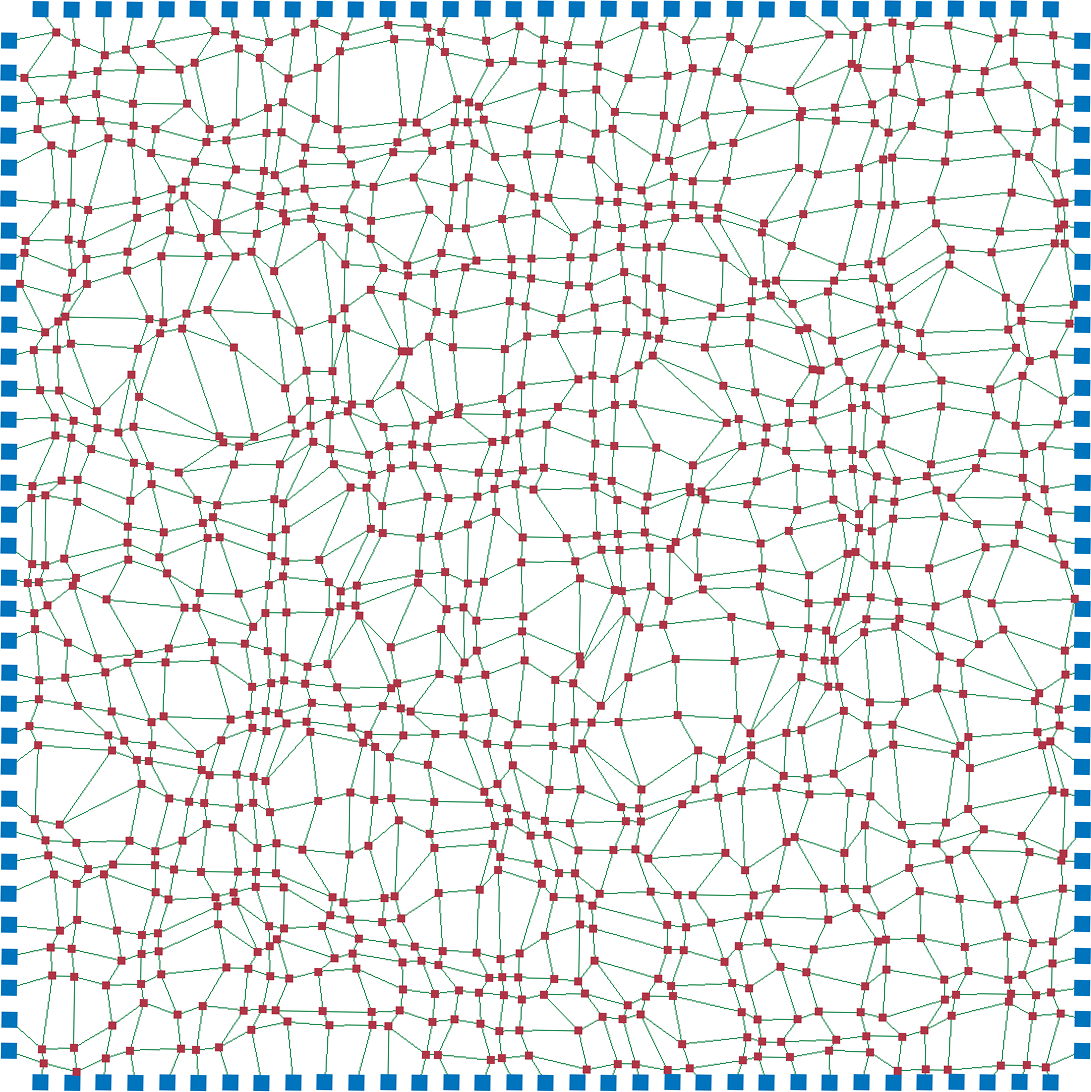
\includegraphics[
		width=\textwidth, 
		height=\textwidth, 
		keepaspectratio=true]
	{./img/results/1200_0_1_highest_97_step_0}
	\caption{Step 0}
	\label{fig:experiment:highestStrain:0}
\end{subfigure}
\begin{subfigure}{0.16\textwidth}
	\centering
	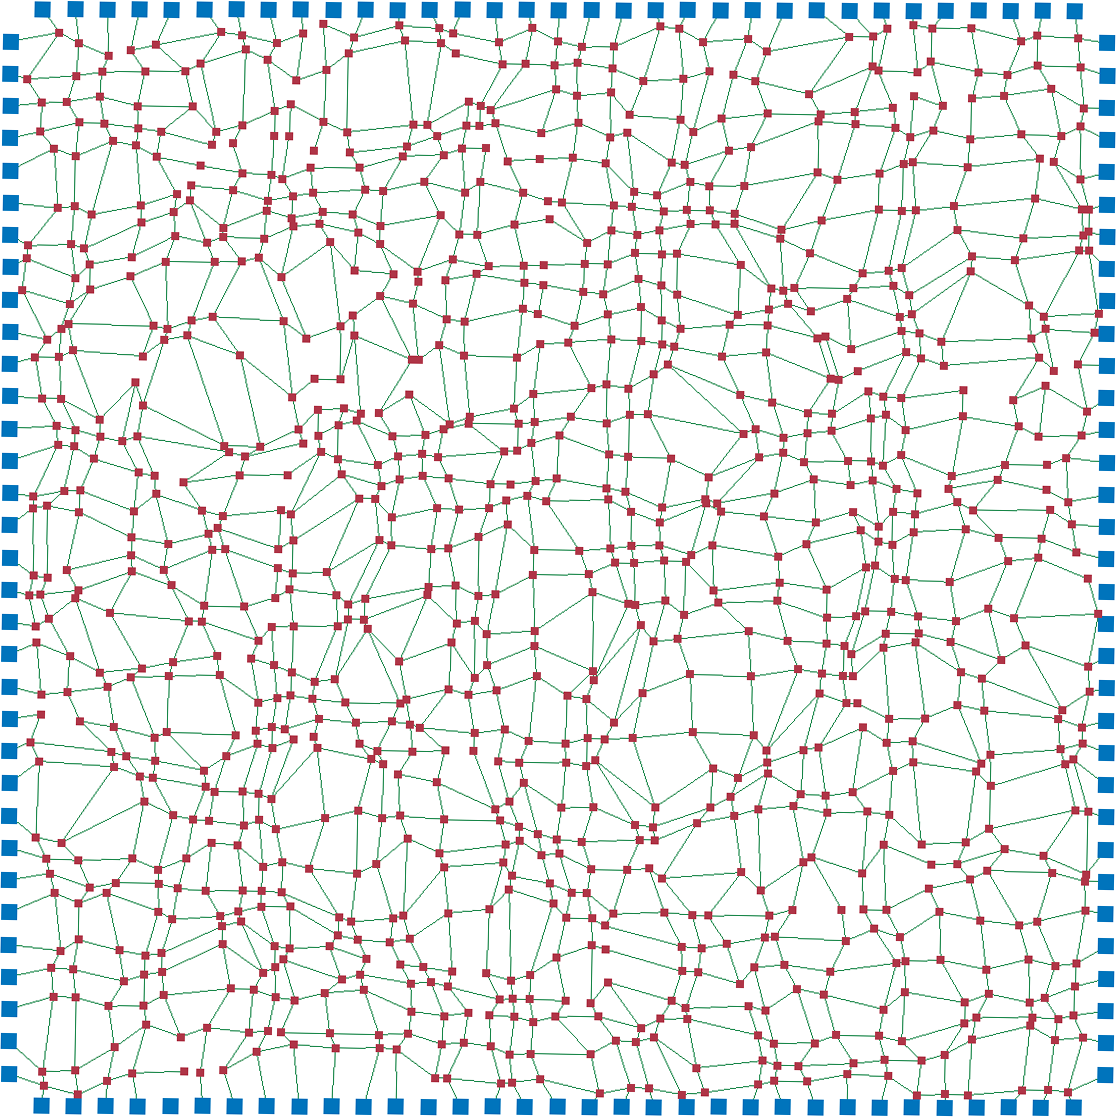
\includegraphics[
		width=\textwidth, 
		height=\textwidth, 
		keepaspectratio=true]
	{./img/results/1200_0_1_highest_97_step_1}
	\caption{Step 1}
	\label{fig:experiment:highestStrain:1}
\end{subfigure}	
\begin{subfigure}{0.16\textwidth}
	\centering
	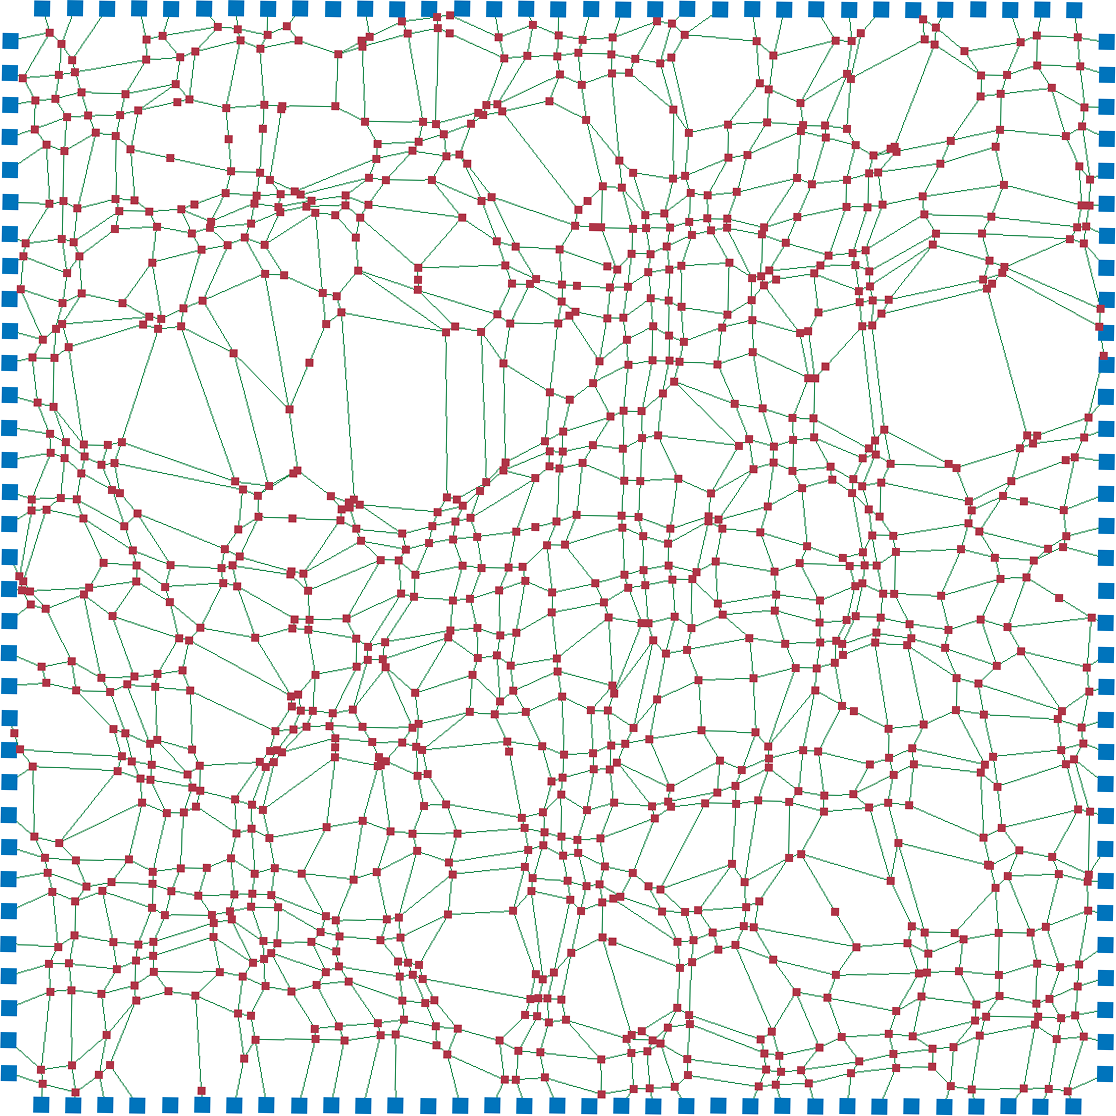
\includegraphics[
		width=\textwidth, 
		height=\textwidth, 
		keepaspectratio=true]
	{./img/results/1200_0_1_highest_97_step_2}
	\caption{Step 2}
	\label{fig:experiment:highestStrain:2}
\end{subfigure}		
\begin{subfigure}{0.16\textwidth}
	\centering
	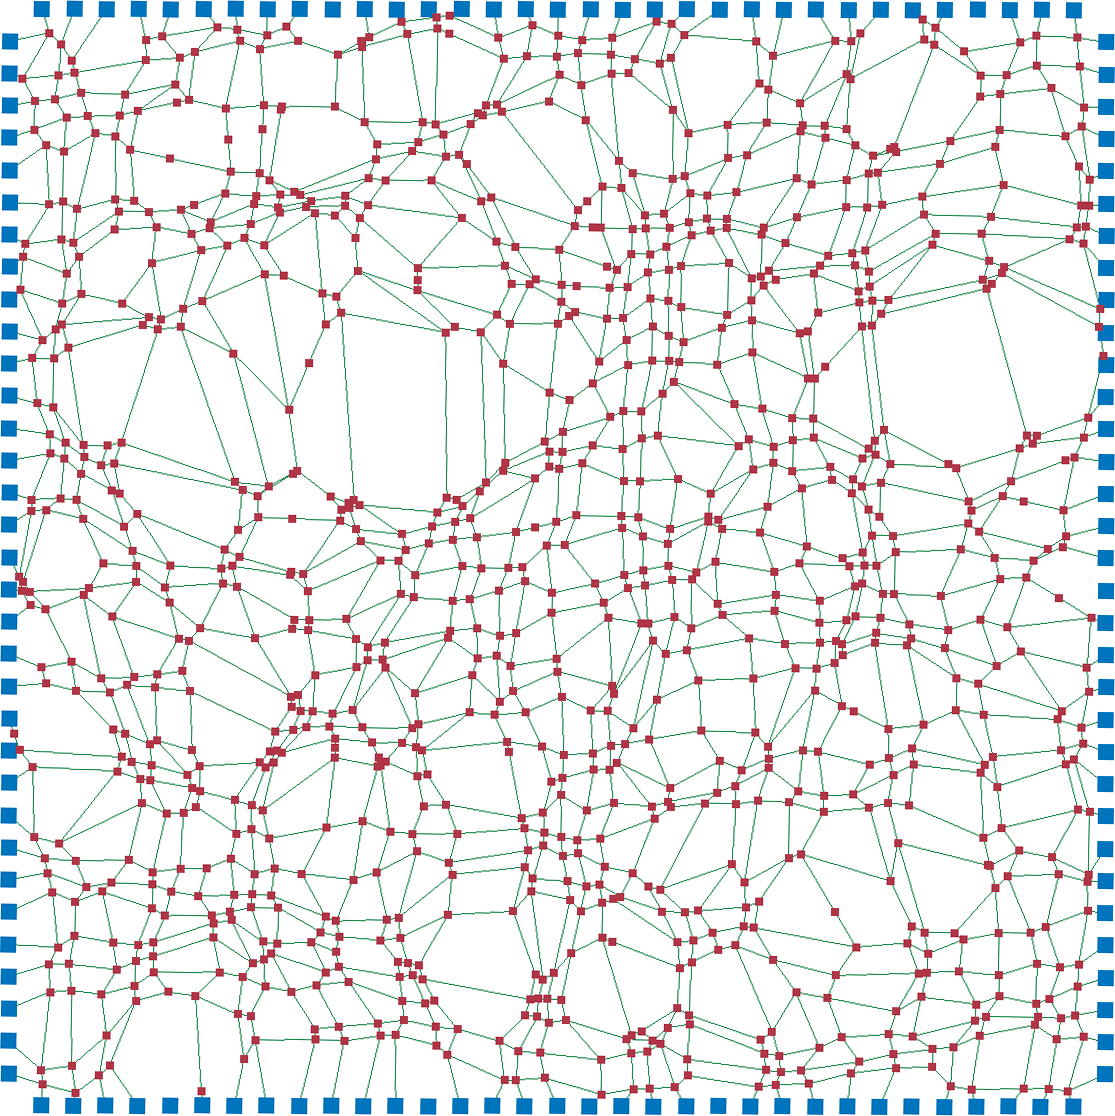
\includegraphics[
		width=\textwidth, 
		height=\textwidth, 
		keepaspectratio=true]
	{./img/results/1200_0_1_highest_97_step_3}
	\caption{Step 3}
	\label{fig:experiment:highestStrain:3}
\end{subfigure}			
\begin{subfigure}{0.16\textwidth}
	\centering
	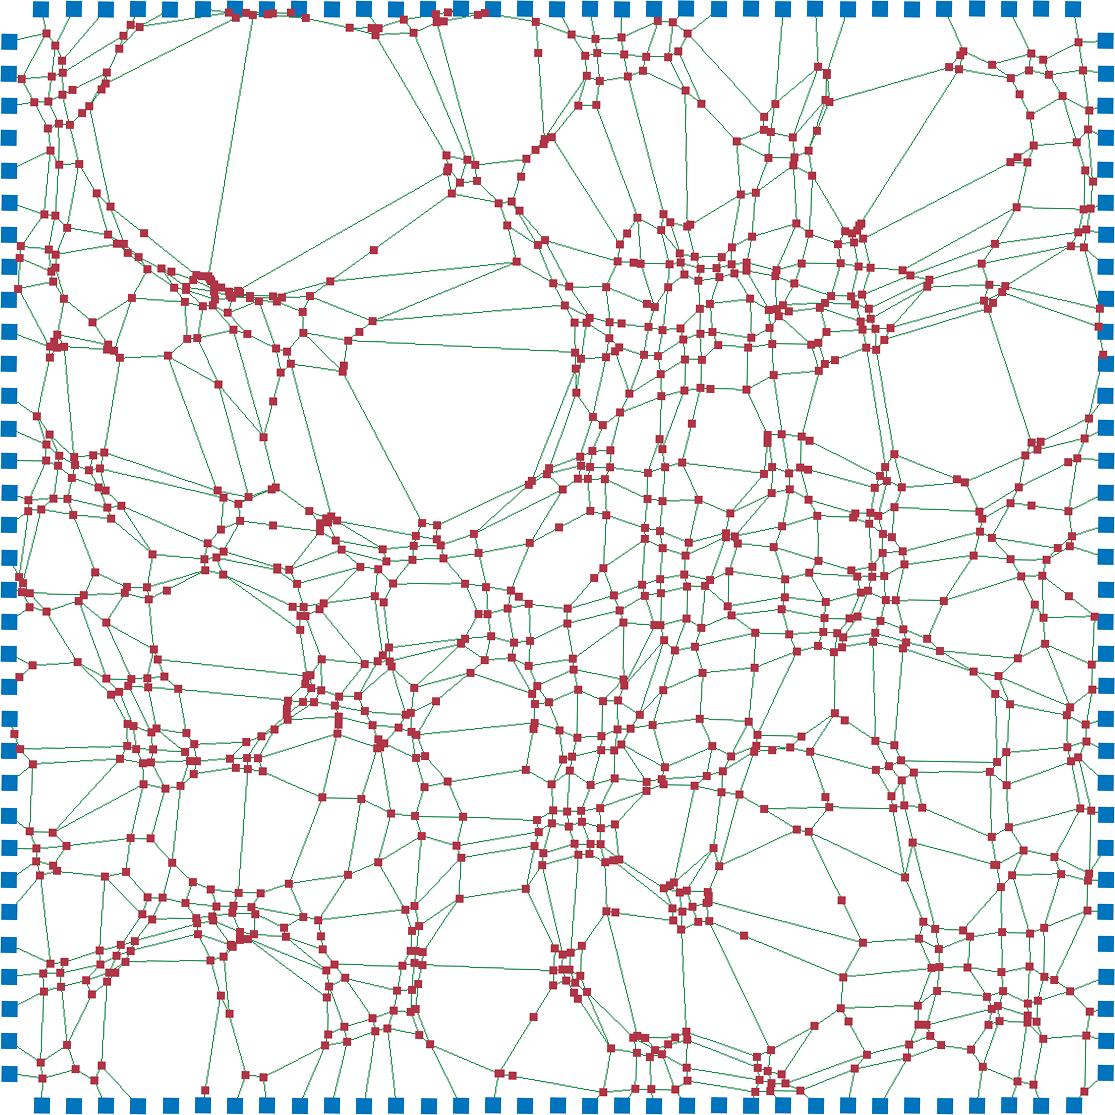
\includegraphics[
		width=\textwidth, 
		height=\textwidth, 
		keepaspectratio=true]
	{./img/results/1200_0_1_highest_97_step_4}
	\caption{Step 4}
	\label{fig:experiment:highestStrain:4}
\end{subfigure}				
\begin{subfigure}{0.16\textwidth}
	\centering
	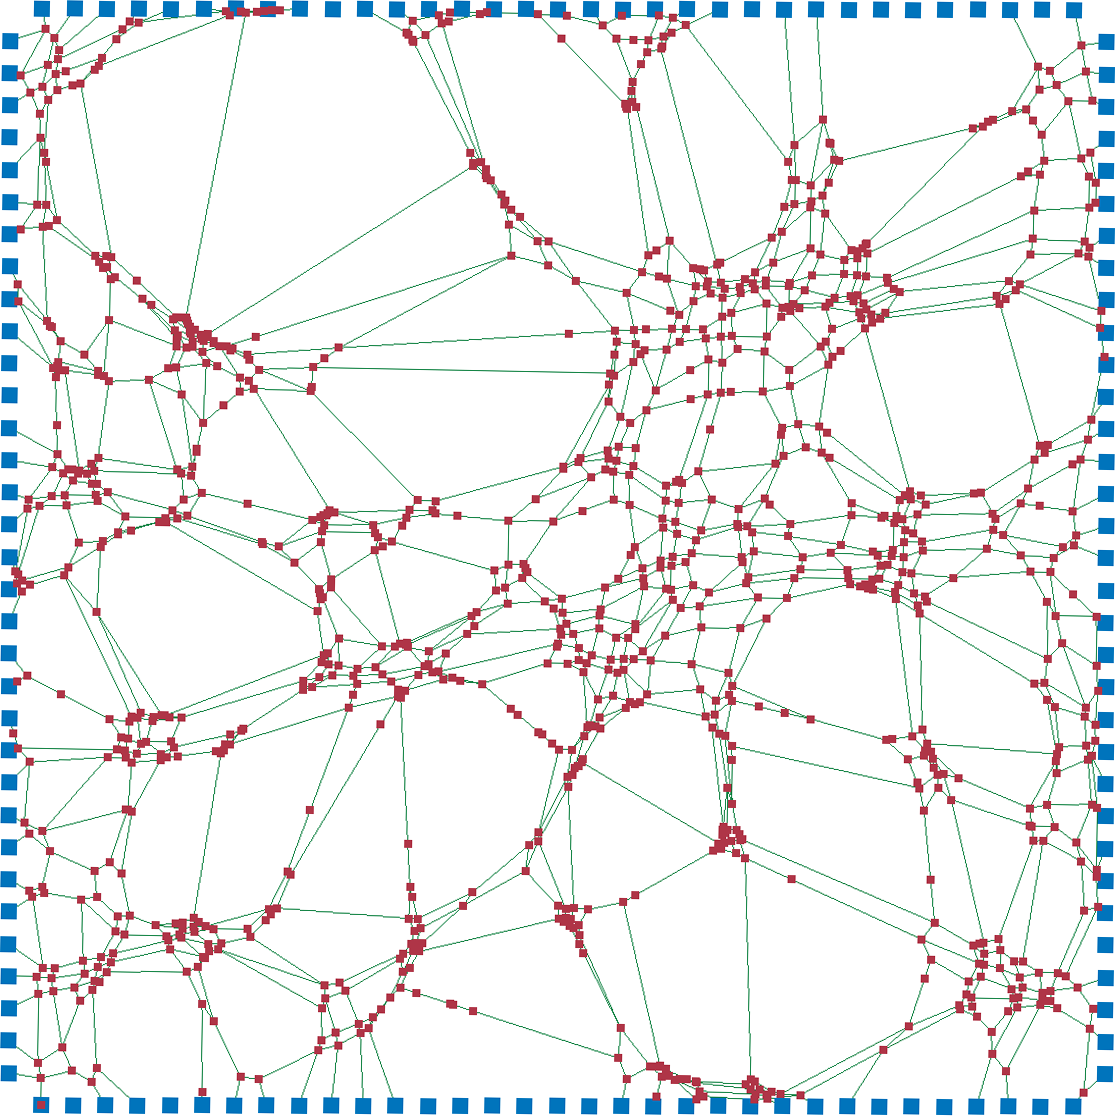
\includegraphics[
		width=\textwidth, 
		height=\textwidth, 
		keepaspectratio=true]
	{./img/results/1200_0_1_highest_97_step_5}
	\caption{Step 5}
	\label{fig:experiment:highestStrain:5}
\end{subfigure}
\begin{subfigure}{0.16\textwidth}
	\centering
	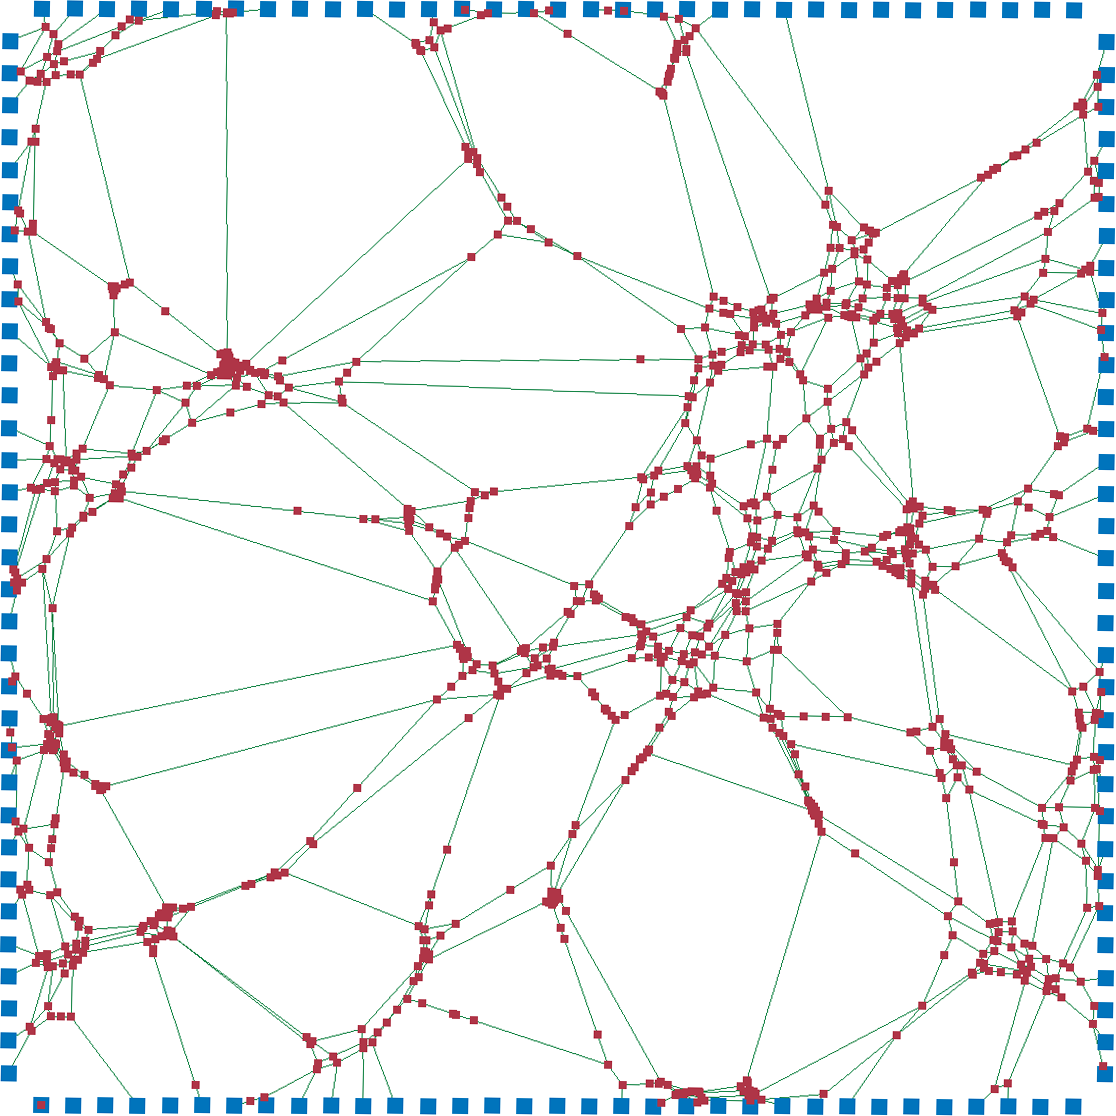
\includegraphics[
		width=\textwidth, 
		height=\textwidth, 
		keepaspectratio=true]
	{./img/results/1200_0_1_highest_97_step_6}
	\caption{Step 6}
	\label{fig:experiment:highestStrain:6}
\end{subfigure}	
\begin{subfigure}{0.16\textwidth}
	\centering
	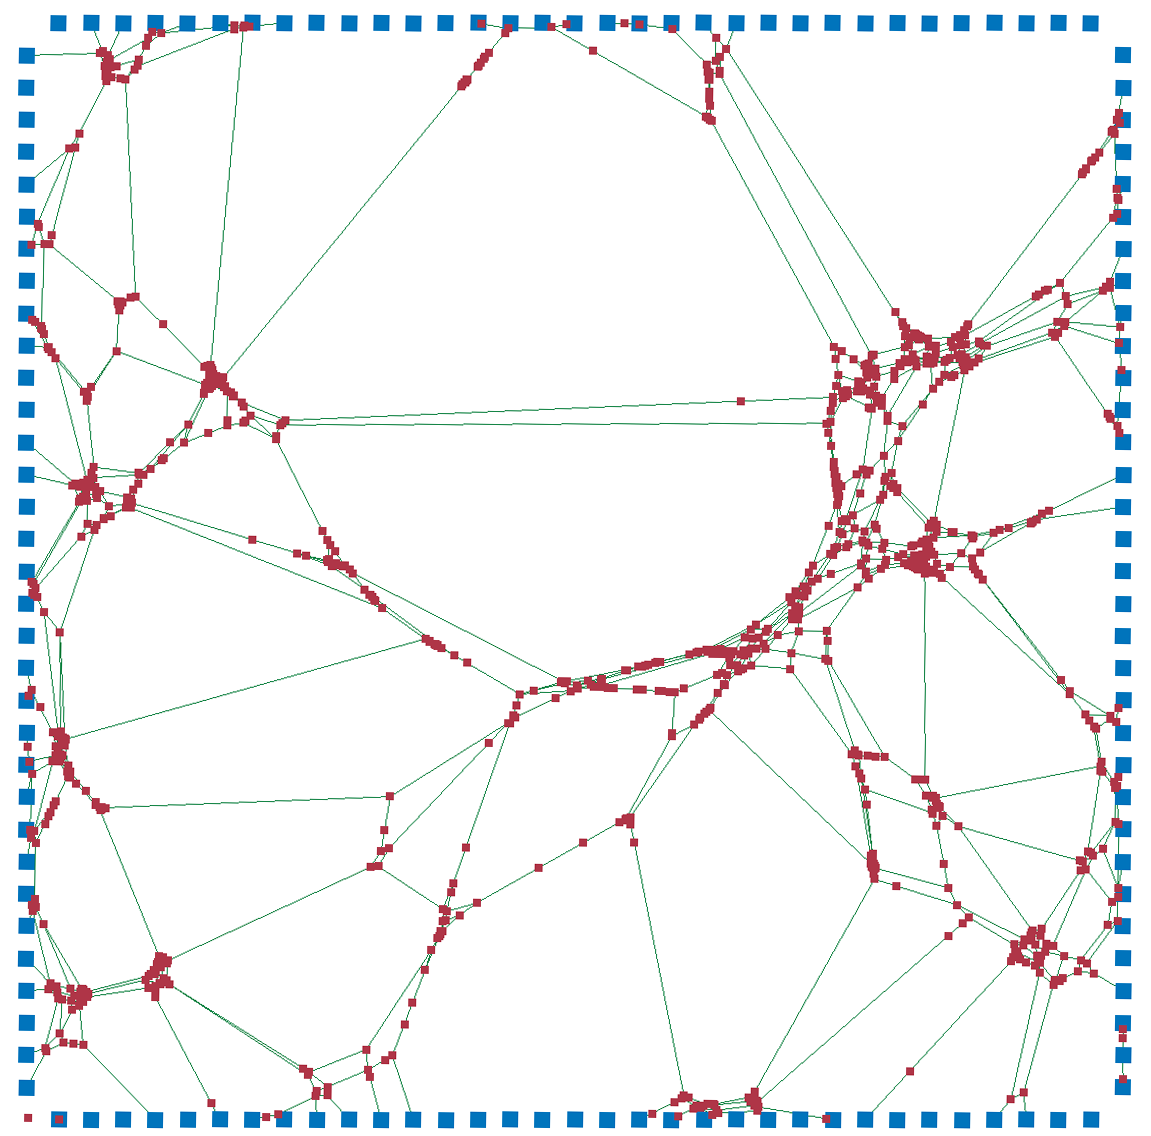
\includegraphics[
		width=\textwidth, 
		height=\textwidth, 
		keepaspectratio=true]
	{./img/results/1200_0_1_highest_97_step_7}
	\caption{Step 7}
	\label{fig:experiment:highestStrain:7}
\end{subfigure}		
\begin{subfigure}{0.16\textwidth}
	\centering
	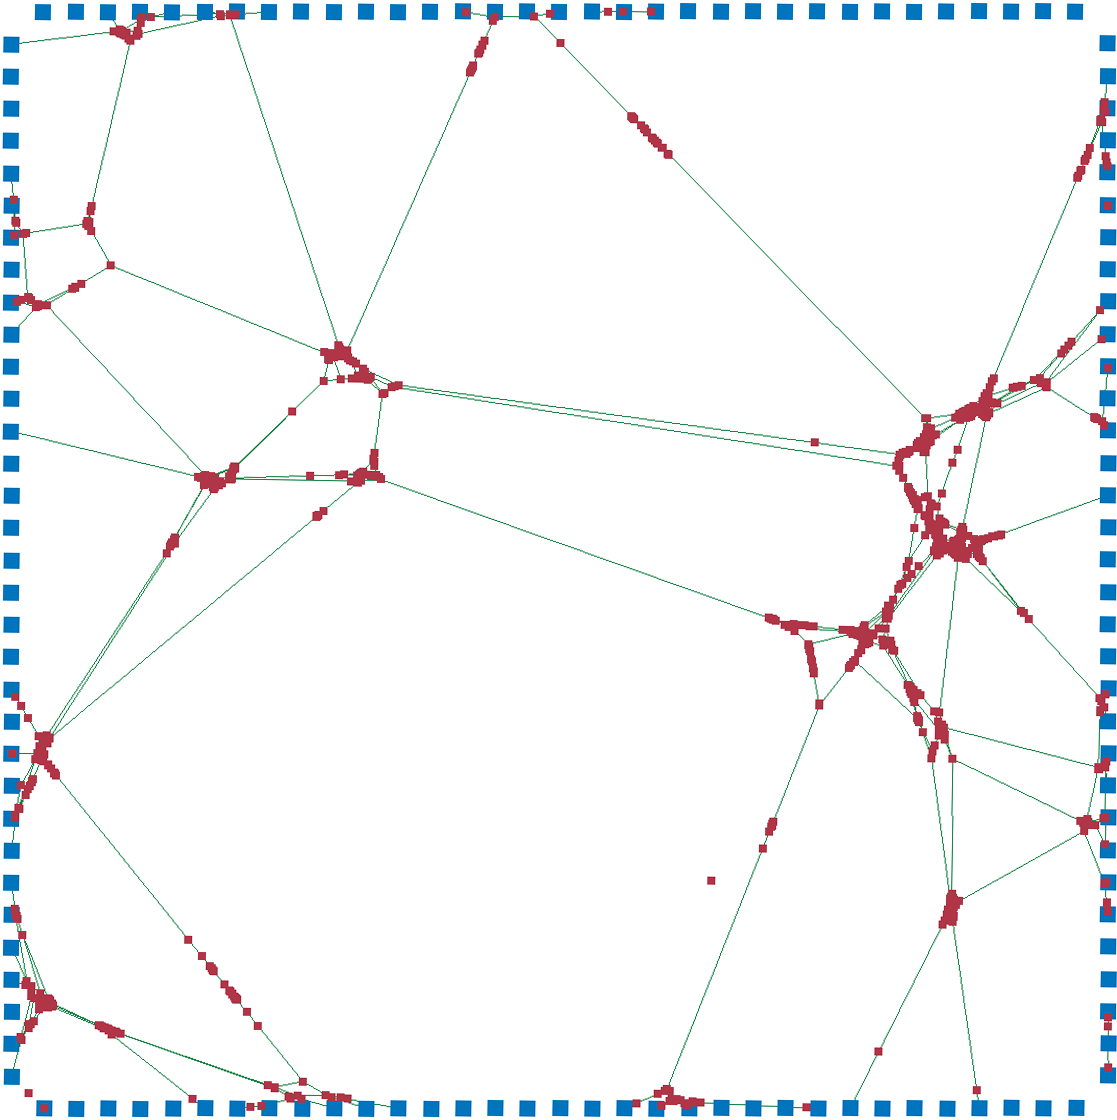
\includegraphics[
		width=\textwidth, 
		height=\textwidth, 
		keepaspectratio=true]
	{./img/results/1200_0_1_highest_97_step_8}
	\caption{Step 8}
	\label{fig:experiment:highestStrain:8}
\end{subfigure}			
\begin{subfigure}{0.16\textwidth}
	\centering
	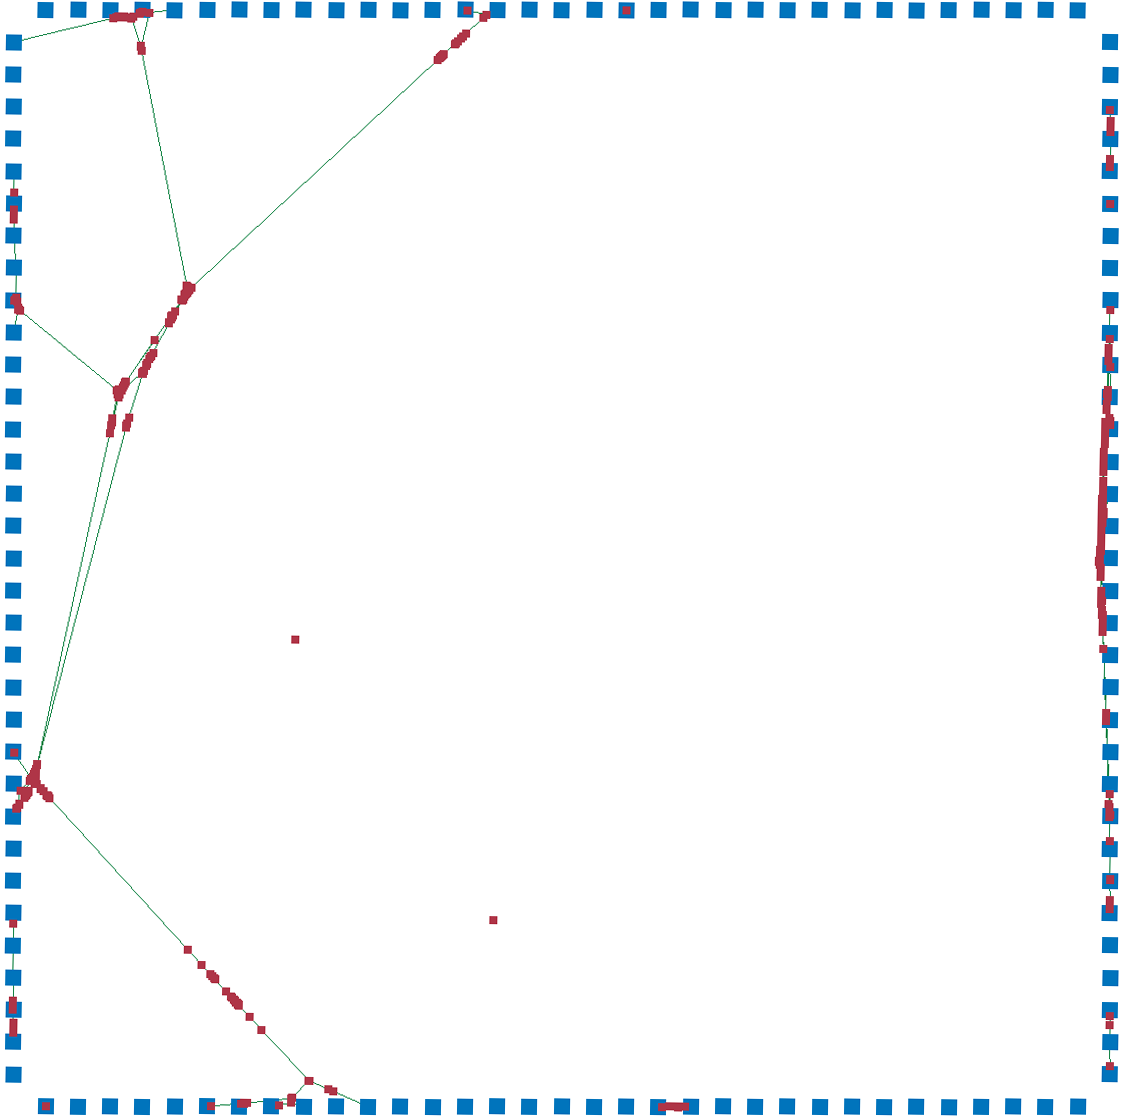
\includegraphics[
		width=\textwidth, 
		height=\textwidth, 
		keepaspectratio=true]
	{./img/results/1200_0_1_highest_97_step_9}
	\caption{Step 9}
	\label{fig:experiment:highestStrain:9}
\end{subfigure}					
\begin{subfigure}{0.16\textwidth}
	\centering
	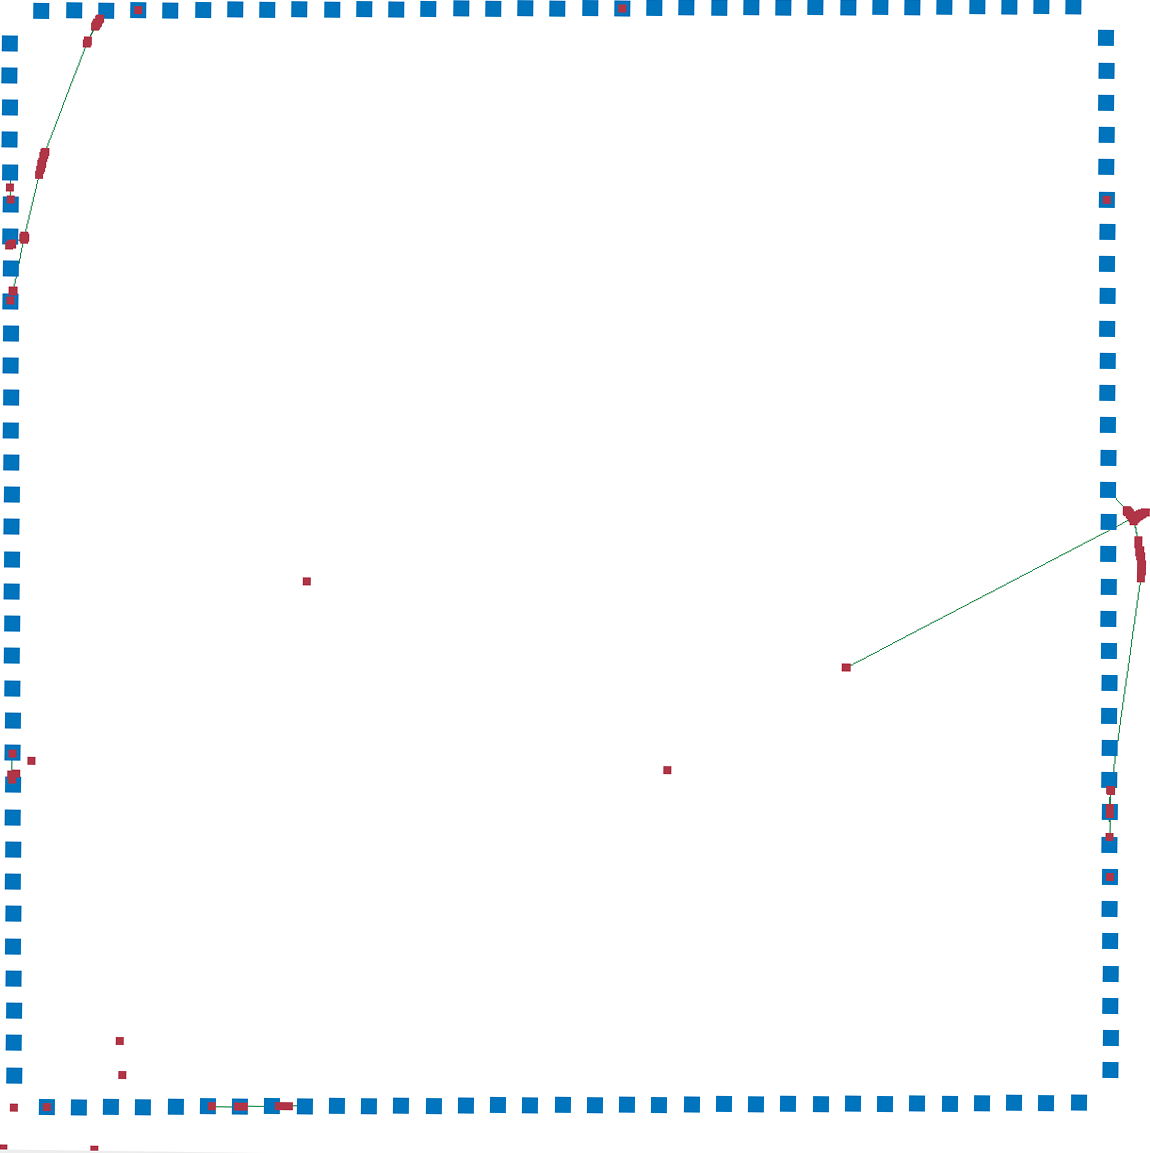
\includegraphics[
		width=\textwidth, 
		height=\textwidth, 
		keepaspectratio=true]
	{./img/results/1200_0_1_highest_97_step_10}
	\caption{Step 10}
	\label{fig:experiment:highestStrain:10}
\end{subfigure}			
\begin{subfigure}{0.16\textwidth}
	\centering
	
\includegraphics[
		width=\textwidth, 
		height=\textwidth, 
		keepaspectratio=true]
	{./img/results/1200_0_1_highest_97_step_11}
	\caption{Step 11}
	\label{fig:experiment:highestStrain:11}
\end{subfigure}						
	\caption{Several steps of the breaking of springs, where the 97 springs with the highest strain were broken. The grid had 1200 particles, the spring constants were sampled from a normal distribution with mean 0.0 and standard deviation 1.0. Step 0 is a stabilization of the initial grid, presented in \cref{fig:implementation:stabilizedInitial}, the following steps are the stabilization and breaking steps of the algorithm.}
	\label{fig:experiment:highestStrain}
\end{figure*}

\begin{figure*}
	\centering
	%!TEX root = report.tex	
\begin{subfigure}{0.16\textwidth}
	\centering
	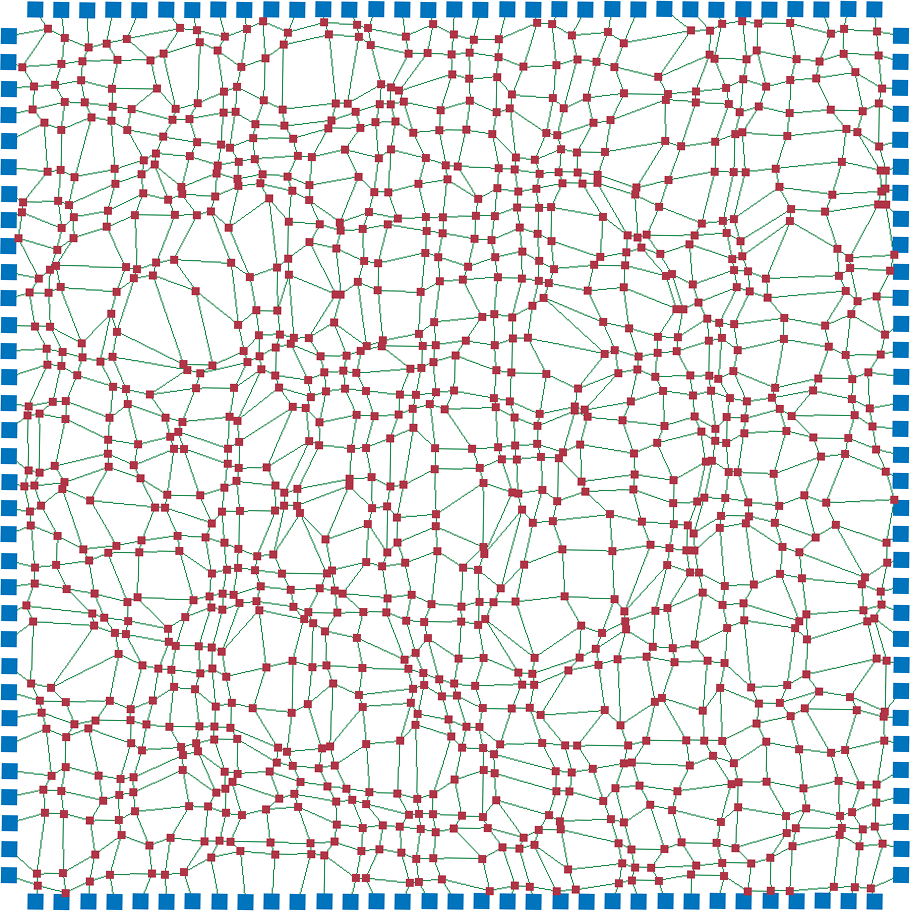
\includegraphics[
		width=\textwidth, 
		height=\textwidth, 
		keepaspectratio=true]
	{./img/results/1200_0_1_greater_104_step_0}
	\caption{}
	\label{fig:experiment:greaterThanStrain:0}
\end{subfigure}
\begin{subfigure}{0.16\textwidth}
	\centering
	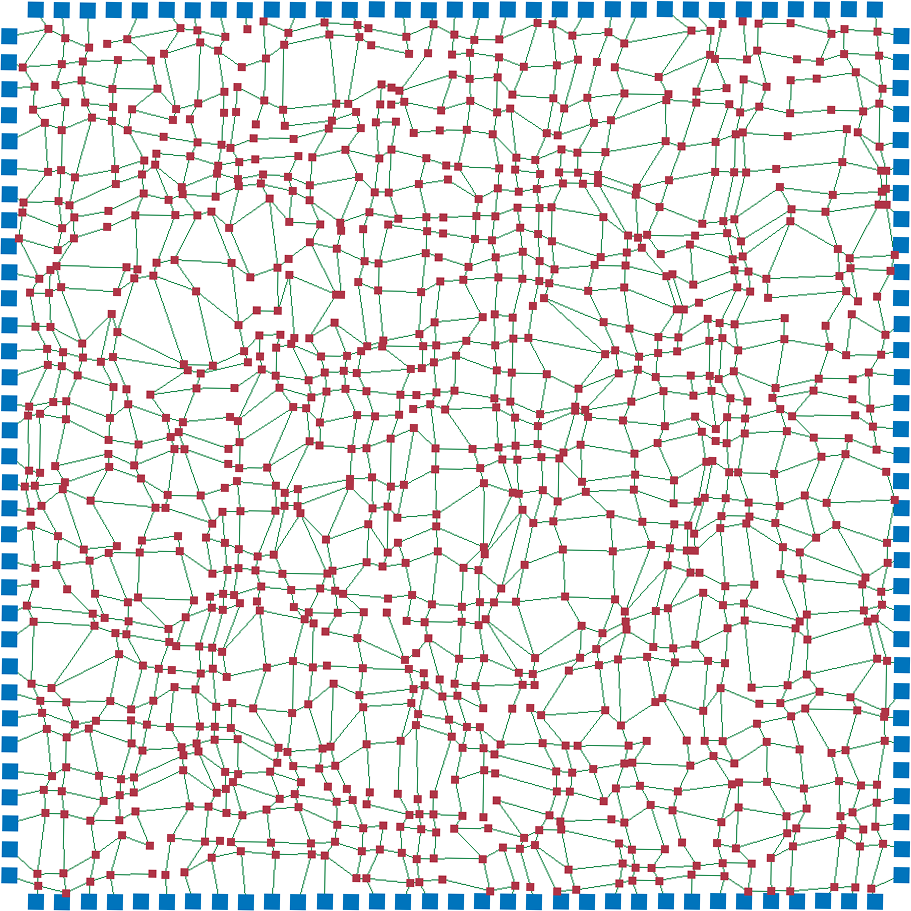
\includegraphics[
		width=\textwidth, 
		height=\textwidth, 
		keepaspectratio=true]
	{./img/results/1200_0_1_greater_104_step_1}
	\caption{}
	\label{fig:experiment:greaterThanStrain:1}
\end{subfigure}	
\begin{subfigure}{0.16\textwidth}
	\centering
	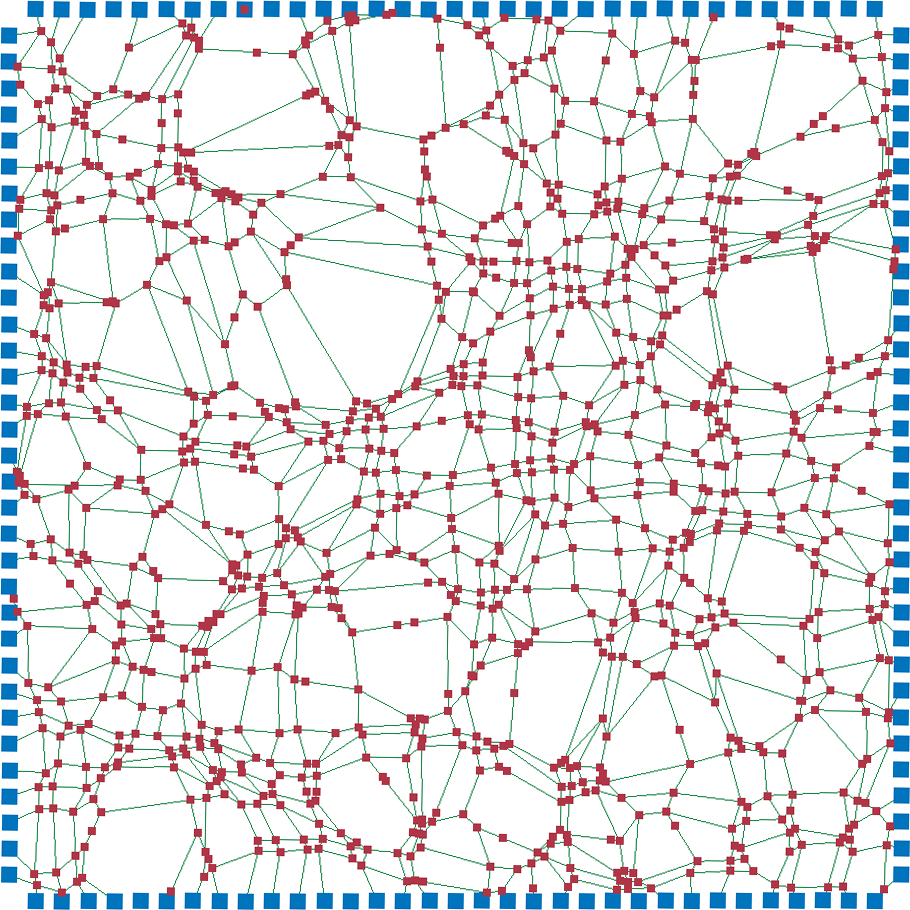
\includegraphics[
		width=\textwidth, 
		height=\textwidth, 
		keepaspectratio=true]
	{./img/results/1200_0_1_greater_104_step_2}
	\caption{}
	\label{fig:experiment:greaterThanStrain:2}
\end{subfigure}		
\begin{subfigure}{0.16\textwidth}
	\centering
	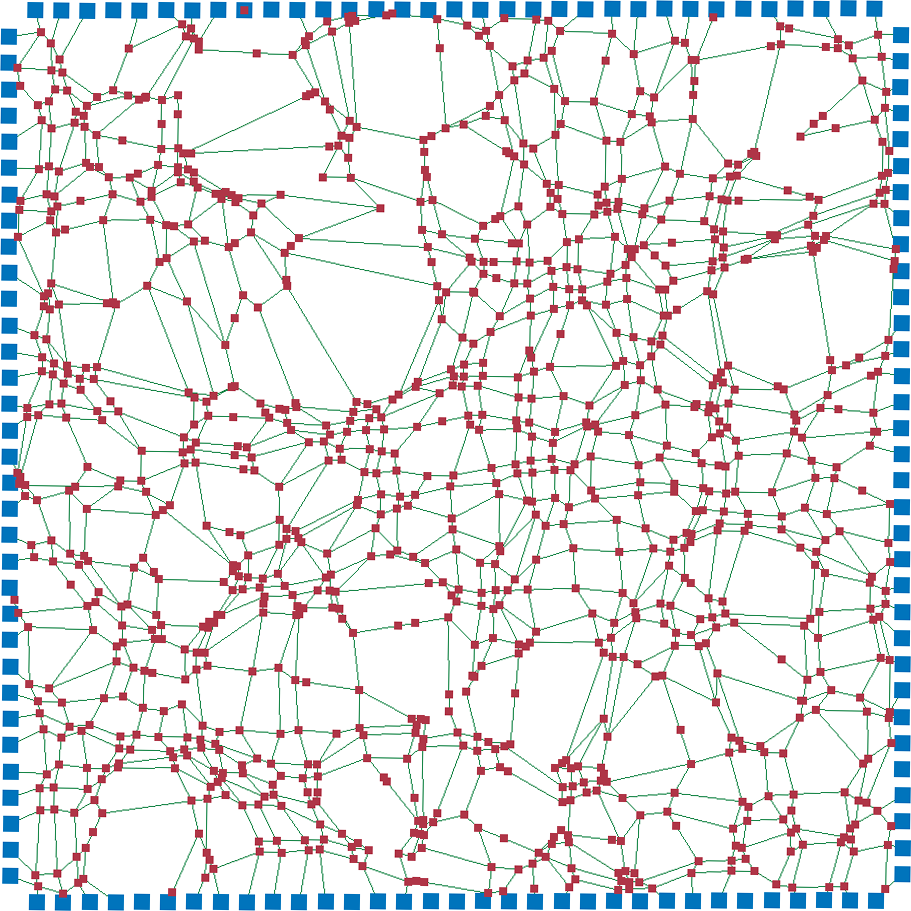
\includegraphics[
		width=\textwidth, 
		height=\textwidth, 
		keepaspectratio=true]
	{./img/results/1200_0_1_greater_104_step_3}
	\caption{}
	\label{fig:experiment:greaterThanStrain:3}
\end{subfigure}			

\begin{subfigure}{0.16\textwidth}
	\centering
	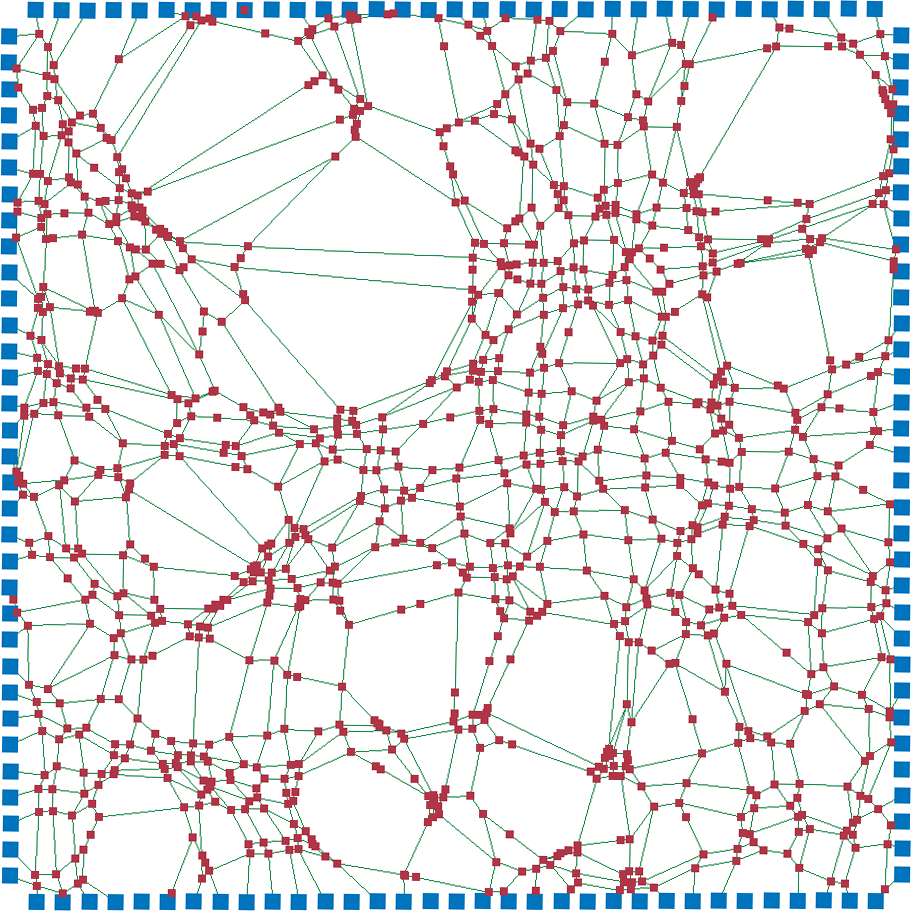
\includegraphics[
		width=\textwidth, 
		height=\textwidth, 
		keepaspectratio=true]
	{./img/results/1200_0_1_greater_104_step_4}
	\caption{}
	\label{fig:experiment:greaterThanStrain:4}
\end{subfigure}				
\begin{subfigure}{0.16\textwidth}
	\centering
	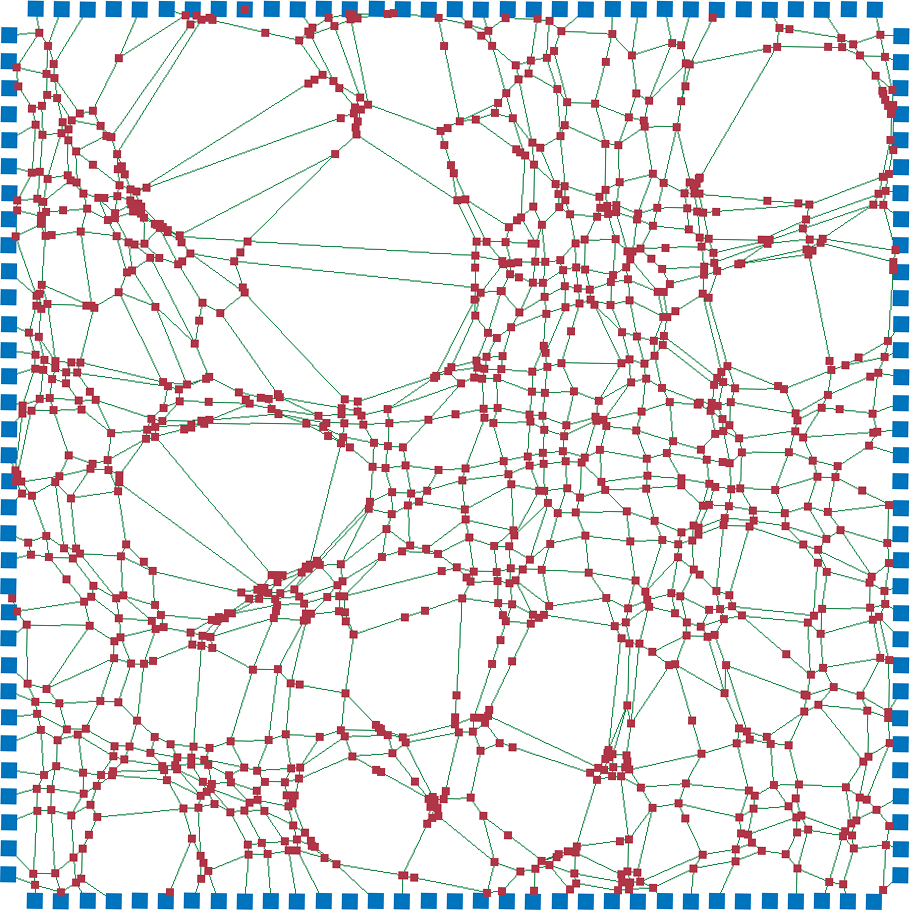
\includegraphics[
		width=\textwidth, 
		height=\textwidth, 
		keepaspectratio=true]
	{./img/results/1200_0_1_greater_104_step_5}
	\caption{}
	\label{fig:experiment:greaterThanStrain:5}
\end{subfigure}
\begin{subfigure}{0.16\textwidth}
	\centering
	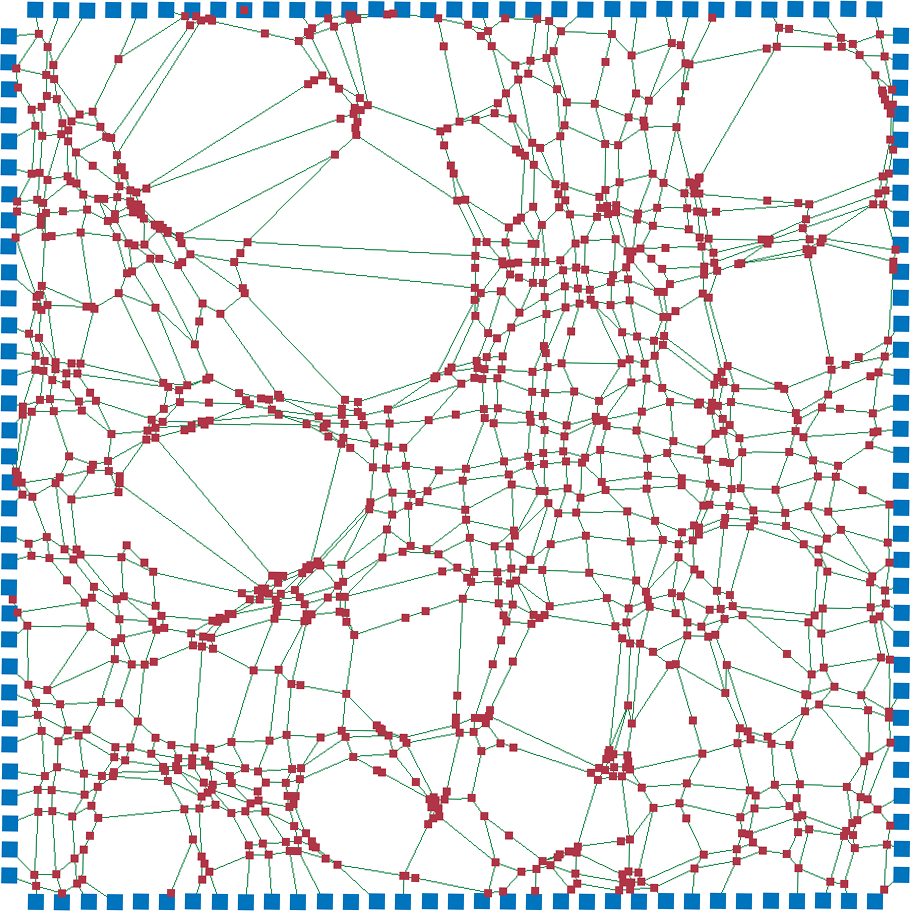
\includegraphics[
		width=\textwidth, 
		height=\textwidth, 
		keepaspectratio=true]
	{./img/results/1200_0_1_greater_104_step_6}
	\caption{}
	\label{fig:experiment:greaterThanStrain:6}
\end{subfigure}	
\begin{subfigure}{0.16\textwidth}
	\centering
	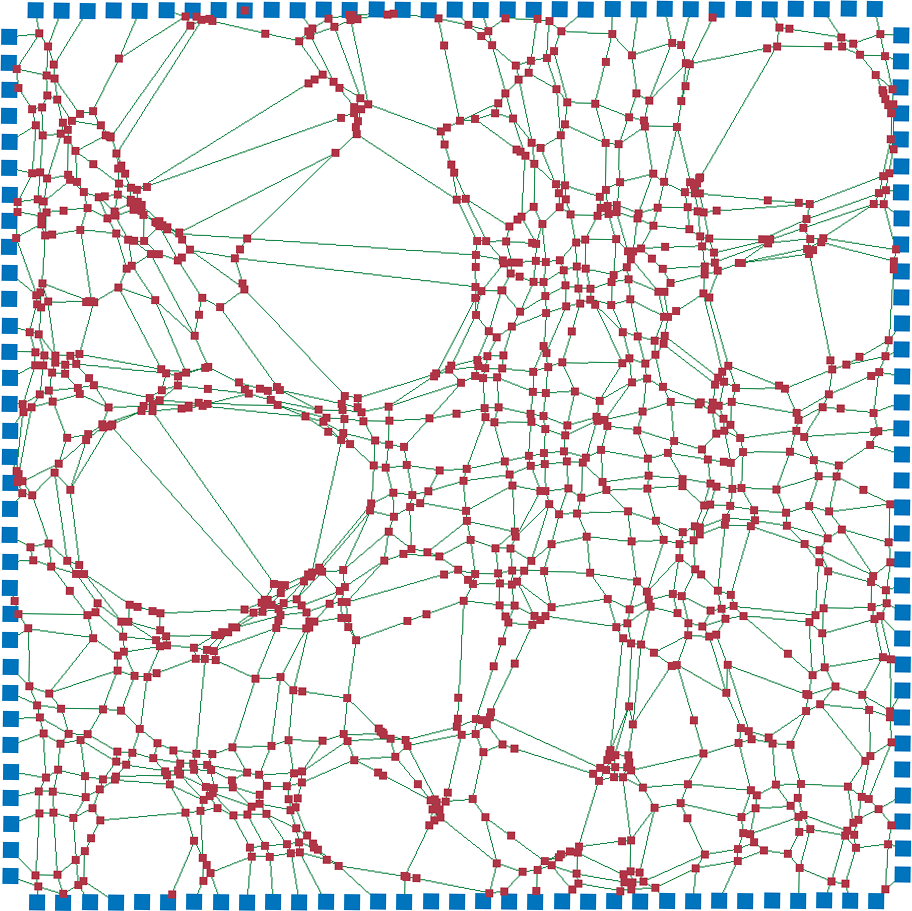
\includegraphics[
		width=\textwidth, 
		height=\textwidth, 
		keepaspectratio=true]
	{./img/results/1200_0_1_greater_104_step_7}
	\caption{}
	\label{fig:experiment:greaterThanStrain:7}
\end{subfigure}							
	\caption{Several steps of the breaking of springs, where the springs with a strain greater than 1.04 were broken. The grid had 1200 particles, the spring constants were sampled from a normal distribution with mean 0.0 and standard deviation 1.0. Step 0 is a stabilization of the initial grid, presented in \cref{fig:implementation:stabilizedInitial}, the following steps are the stabilization and breaking steps of the algorithm.}
	\label{fig:experiment:greaterThanStrain}
\end{figure*}	

% \section{Discussion}
% %!TEX root = report.tex

\todo[inline]{Deeltje dat met maar een veertje vast zit gedraagt zich raar. Mogelijke oplossingen. Gevolg: balon effect}

\section{Conclusion}
\label{s:conclusion}
%!TEX root = report.tex

\todo{The conclusion, i.e., (depending on if we extend our implementation to include more options then now) In short: Our method is fast but (without fixed particles to the ground, maybe?) does not model the rupturing of mud. (How are we going to measure fast?)}



\printbibliography

\end{document}